\documentclass[11pt]{article}

%% Language and font encodings
\usepackage[english]{babel}
\usepackage[utf8x]{inputenc}
\usepackage[T1]{fontenc}

%% Sets page size and margins
\usepackage[a4paper,top=1.5cm,bottom=1.5cm,left=2cm,right=2cm,marginparwidth=1.75cm]{geometry}

% One inch margins
%\PassOptionsToPackage{margin=0.5in}{geometry}

% Add extra blank line between paragraphs, and remove paragraph indentation
\usepackage[parfill]{parskip}
\parskip = 0\baselineskip

% Single spacing
\usepackage{setspace}
\setstretch{1}

%% Useful packages
\usepackage{amsmath}
\usepackage{graphicx}
\usepackage{booktabs}
\usepackage[colorinlistoftodos]{todonotes}
\usepackage[colorlinks=true, allcolors=blue]{hyperref}

\title{Group I Final Paper: Deep Learning Stock Volatilities with Google Trends}
\author{Group Member: Tian Ye, Yuanyi Liang, Chengyue Zhang, Ke Peng}

\begin{document}
\maketitle

\section{Introduction}

In quantitative trading, it is crucial to find out the underlying relationships between the time series or predict future values so that we can generate trading signals. Many research has been done using machine learning methods and recurrent neural networks (RNNs) to forecast financial time series. However, there are limited studies conducted about Artificial neural networks (ANNs). Recent analysis has shown the advantages of ANNs as good nonlinear function approximators. The Long Short-Term Memory (LSTM) network is a type of recurrent neural network that used in deep learning. It keeps a context of memory within the pipeline, and has the ability to deal with the issue of exploding and vanishing gradient.

\vspace{5mm}

In building prediction models, many studies have used sentiment analysis of social media and text mining, such as analyzing Twitter information or live news feeds to forecast stock prices or volatility. Some research has also looked at the predicting power of unemployment, consumption and other macroeconomic indicators using data of Google search. In this work, we utilize a larger scale data of Google Trend to predict market volatility. Google Trends is a website by Google that analyzes the popularity of top search queries in Google Search across various regions and languages, which represents public interests through more key terms. 

\vspace{5mm}

In this paper, we mainly focused on using LSTM and GRU model to regress and predict market volatility, incorporated with Google Trends as well as market data. Then we built and tested several trading strategies to applied those prediction into market trading.

\vspace{5mm}

In the following three sections, we introduced the process of collecting Google Trend data, refining Neural Network architecture and designing trading strategies. At last, we will give a conclusion about the contribution of Google Trend data in predicting volatility, performance of different model structures and different trading strategies.

\section{Google Trend Data Retrieval}
\subsection{Select 10 key words}

According to the paper, \textit{Quantifying Trading Behavior in Financial Markets Using Google Trends} (2013)~\cite{bib1}, Google Trends data reveal human behavior in some senses. The complex human behavior might affect financial markets and led to crises. The paper suggests that Google Trends data may provide some insight into future trends of the economic actors’ behavior. For instance, before the trends that people tend to sell at lower prices on the financial market, they might be really concern and tend to search for more information about the market status. This can be reflected by Google Trends search volumes change for words related to the markets.

\vspace{5mm}

The paper investigated 98 words and their relationship with trader decisions. Based on the return ranking of those 98 investigated search terms for hypothetical trading strategies, we selected the following ten potential key words for our analysis: color, markets, unemployment, revenue, housing, portfolio, inflation, economics, debt, stocks.

\subsection{Run codes}

Google decides the granularity of the resulting data based on the time frame we used for searching. The maximum time rage for daily data is 3 months. Anything longer than that would only give us weekly or even monthly data. However, for the use of our model, we need daily trend data for about 13 years. Extracting those trend data directly would only return monthly data. Therefore, we decided to split the whole time-frame into several smaller ones, which are 90 days in our case, and keep a one day overlap in between so that we can normalize the scale for the data of those small segments. 

\vspace{5mm}

Google Trends daily data represent search interest on specific day relative to the highest day within the same search period. For the highest day, Google Trends sets the number for that day to be 100, and the values for other days in the same search time frame are scaled relative to that amount. Thus, in order to concatenate the trend data and get daily data for the entire selected time range, we need to rescale the data together.

\vspace{5mm}

The codes we used to retrieve and process Google Trends data are adjusted from the codes that Malik Koné~\cite{bib2} posted on GitHub. The program uses Pytrends, an API for Google Trends, to download trend data reports from Google. Firstly, the codes connect to Google and build an array of 90 days periods with one day resolution. To get the rescaled data for the whole time-range, we need one more than the number of 90 days within the selected time frame. If the end time been entered is in the future, Google returns the most recent data. Then the program loops through all the words in the key word list to get trend data for each word. Before concatenation, a multiplication factor is calculated by using the search interest score number of the overlap day in the previous concatenated data array to divide the number of that day in the latter period. The program utilizes this multiplication factor to rescale and concatenate the data. Finally, the data would be adjusted into csv files, and stored for later use of our model.

\section{RNN Model Structure Refine}

We referred to paper \textit{Deep Learning Stock Volatility with Google Domestic Trends} (2015)~\cite{bib3} in the project. The paper used a LSTM layer and a DNN layer to regress market volatility in the next day using S\&P500 return, volatility, Google trend data in the past 10 days. Code implemented by Keras was presented in GitHub. Our work primarily focused on modifying Keras format to Tensorflow, strengthening model robustness and adding rolling window. Following shows our process in details.

\subsection{Implement Tensorflow Structure}

We applied two classes to implement  the regression neural network. One class defines LSTM architecture, while the other fits the given neural network in the training set and predicts volatility in the test set.

\vspace{5mm}

After replicating the paper~\cite{bib3}, we compared the results run by Keras and Tensorflow (see figure 1 and figure 2 in appendix). We discovered that iteration epochs and performance under two structures are different. Keras version converged after 6000 epochs while Tensorflow version didn't achieve until 50000 epochs. Besides, Tensorflow version underperformed Keras version a little bit in the test set. Possible reasons include different initializer and different graph nodes.


\vspace{5mm}

We observed that Tensorflow program we designed is a straight forward node from LSTM, DNN (sigmoid activation) to DNN (linear activation), while that of Keras are much more complicated. This is the main reason that we can not replicate the result exactly.


\subsection{Strengthen RNN robustness}

In a ten-year framework with daily S\&P500 and Google trend data, we only have 2122 training data and 616 testing data, which is small compared with original nodes of each layer proposed by the paper (32 in LSTM and 16 in DNN). We encountered overfitting and instability issues as training epochs get greater and different initializer. Therefore, we decided to reduce parameters by cutting down nodes from (32,16) to (16,8) within each layer. We also replace LSTM layer with GRU layer, which has similar function but less parameters. Both methods achieved stableness after 20000 training epochs.

\subsection{Add rolling window}

In the original paper, the authored only trained one model to predict volatility in the next three years, leading to a decrease of MAPE in the last part of the testing period. To improve model performance in the test set, we applied a rolling window of training size 2000 for each 100 days. This allows the model to update sentiment in a period and reaches a better result.

\section{Trading Strategy}

\subsection{Naive Strategy}

In order to take advantage of volatility prediction we have finished, we applied it to trade asset in the market. The first step was to replace volatility with VIX index considering real market practice. The next step was to find a tradable asset that has high correlation to VIX index. We chose VXX index as our asset because it is a combination of VIX futures and it doesn't need to roll over every month. Our strategy trade 1 dollar value of VXX index on a daily basis. If the predicted VIX index is higher than today's value, then we will buy VXX index. On the contrary, if the predicted VIX index is lower than today's value, then we will sell VXX index. In this strategy, we are betting the predicted direction of volatility and the correlation between VIX and VXX index. 

\vspace{5mm}

Since we have confidence in predicting VIX index value (as we can see from figure 3 in the appendix plotting observed VIX and predicted VIX), we earned profits in days when we get the direction correct (P\&L see figure 4 in the appendix). For the VIX index, accuracy of prediction is 57.63\%, and the accuracy for VXX index is 58.28\%. In the back-testing period (April 2015-October 2017), we achieved about 3 dollar return for 1 dollar invested without considering transaction cost. If we set transaction cost as 10 basis point per trade, we still have about 240\% profit in the 600 days.

\vspace{5mm}

Above result is achieved by GRU layer with 32 nodes and dense layer with 16 nodes. Features used here are the past 10-days' S\&P500 return, VIX index value and Google Trend Data of keyword 'computers \& electronics'.

\subsection{Strategy Improvement}

For the naive strategy, we are predicting the value of VIX index and then form our trade of VXX based on comparison between the prediction and today's VIX index value. There are three possible steps to make the improvement.

\vspace{5mm}

First, we can change the model to have a binary classification output instead of the a predicted value so that we are directly focusing on predicting the direction of VIX index movement and have a better accuracy. For a binary classification model, we do not need to modify the model structure. In the training part, we should change our loss function from MAPE to sigmoid cross entropy. For the prediction part, we apply a sigmoid function to the logit value obtained from the network and set the threshold to be 0.5. Also, the training epoch is changed to 1500 for the binary classification task in order to prevent overfitting. We get this training epoch number by running more iterations at first and then choose the training epoch to have the highest accuracy on the validation set. These modification do improve the prediction accuracy of VIX index on test set from 57\% to 69.5\%. However, the performance of the strategy decreases a little bit with smaller cumulative return (about 80\% during the same period before transaction cost) and larger volatility and drawdown. 

\vspace{5mm}

For the first improvement, we are trading VXX but we are still making a direction prediction for the VIX index. As a result, we are not only betting the direction but also the correlation between VXX and VIX index. In order to eliminate the bet on correlation, we change our prediction target to be the direction of VXX price change. We also add the past values of VXX into our feature set. Since VXX data is only available from 2009/01/30, the starting date of the training period should be changed to this date. We keep the test period unchanged. For the original VIX prediction, we smooth the series by taking a moving average of the original or squared series. Here, we skip this smoothing operation to make the series reflect more real-time change. We use the past 10 values of VXX, VIX index and S\&P 500 returns as features and train the model. At this time, the prediction accuracy on test set is 58.4\%, which is a very good result for daily strategy. The performance of the strategy is also very good (see Figure 5) with about 250\% cumulative return during the same period before transaction cost. The volatility and drawdown is also small for this strategy.

\vspace{5mm}

Since the general trend of VXX is going down in the test period, we compare our improved strategy with the short and hold strategy (take short positions on all days, see Figure 6). The result shows that these two strategies have similar performance. However, our improved strategy have larger cumulative return with larger gain when the strategy works well and smaller drawdown when the strategy loses money.

\vspace{5mm}
The third possible step of improvement is to add our retrieved Google Trend data as features. We add one potential keyword at each time to the existing three features to see whether the keyword can add value to the prediction and strategy. In terms of prediction accuracy (See Table 1), adding any one of the keyword does not improve the accuracy significantly. As for strategy performance, we tend to have similar return pattern for adding keyword. However, none of the keyword lead to a better performance in terms of cumulative return and drawdown. One possible explanation is that the overlap between people searching stuffs on Google and people trading in the market might be small. Also, the increase in volatility tends to have different causes at each time. Thus a single keyword or a single topic can not be representative all the time.

\begin{table}[htbp]
  \centering
  \caption{Prediction Accuracy for Adding One Keyword at A Time}
 \scalebox{0.8}{%
    \begin{tabular}{|l|c|c|c|c|c|c|c|c|c|}
    \toprule
    \textbf{Keyword} & \multicolumn{1}{l|}{\textbf{color}} & \multicolumn{1}{l|}{\textbf{debt}} & \multicolumn{1}{l|}{\textbf{economics}} & \multicolumn{1}{l|}{\textbf{housing}} & \multicolumn{1}{l|}{\textbf{inflation}} & \multicolumn{1}{l|}{\textbf{markets}} & \multicolumn{1}{l|}{\textbf{revenue}} & \multicolumn{1}{l|}{\textbf{stocks}} & \multicolumn{1}{l|}{\textbf{unemployment}} \\
    \midrule
    \textbf{Accuracy} & 59.70\% & 59.10\% & 56.70\% & 59.10\% & 59.70\% & 57.60\% & 57.00\% & 57.10\% & 58.00\% \\
    \bottomrule
    \end{tabular}%
 }
  \label{tab:addlabel}%
\end{table}%


\vspace{5mm}


\section{Conclusion}

In this project, we started from a paper to predict market volatility using Google Trend data and extended it to a tradable strategy. We first unfolded process of building and training Recurrent Neural Network by rewriting code in Tensorflow and comparing performance with Keras format. After that, based on our observation of model results, we strengthened the robustness of Neural Network by reducing parameters of LSTM layer and substituting it with GRU layer. They provided excellent MAPE results when predicting the value of volatility. Since volatility is an important measure of market sentiment, as financial engineers, we hoped to extend the prediction to actual trading strategy. First of all, we applied VIX index as volatility measure. However, VIX index is not a tradable asset. Therefore, we tried to trade other assets that have high correlation with VIX such as VXX and VIX futures. The fact is that VIX products continue to decrease over the period while index sometimes spikes. We also trained VXX index directly and obtained good results. At last, we tested the significance of new Google Trend keyword and found that there is no direct connection between searching volume and volatility spike. Market volatility can be sufficiently predicted by the past 10 day's S\&P500 return and volatility.

\vspace{5mm}

As for the strategy part, we need to continue to explore contracts whose values are highly sensitive to VIX index. Another direction would be turn the predicted value of volatility into trading signals by certain formula.

\begin{thebibliography}{10}

\bibitem{bib1}
Preis, T., Moat, H. S., \& Eugene Stanley, H. (2013)
\newblock {{Q}uantifying Trading Behavior in Financial Markets Using Google Trends}.
\newblock \emph{Scientific Reports, 3}. https://doi.org/10.1080/10888438.2015.1057824

\bibitem{bib2}
Koné M. (2018, January 7).
\newblock Retrieved from https://github.com/GeneralMills/pytrends/issues/174

\bibitem{bib3}
Xiong, Ruoxuan, Eric P. Nichols, and Yuan Shen. 
\newblock{Deep learning stock volatility with google domestic trends}. 
\newblock \emph{arXiv preprint arXiv:1512.04916 (2015).}


\end{thebibliography}

\newpage
\appendix
\section{Appendix}

\begin{figure}[htbp]
\centering
\begin{minipage}[t]{0.48\textwidth}
\centering
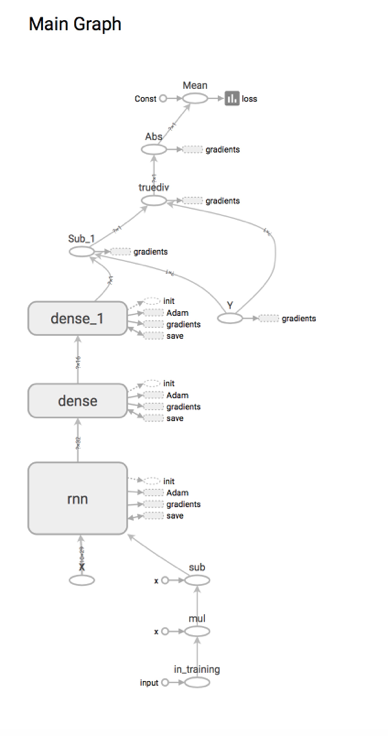
\includegraphics[width=6cm]{Picture1.png}
\caption{Tensorflow graph nodes}
\end{minipage}
\begin{minipage}[t]{0.48\textwidth}
\centering
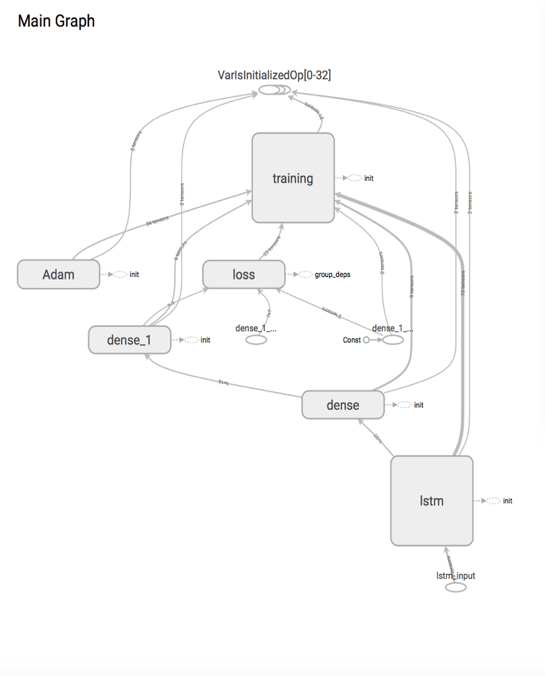
\includegraphics[width=6cm]{Picture2.png}
\caption{Keras graph nodes}
\end{minipage}
\end{figure}

\begin{figure}[htbp]
\centering
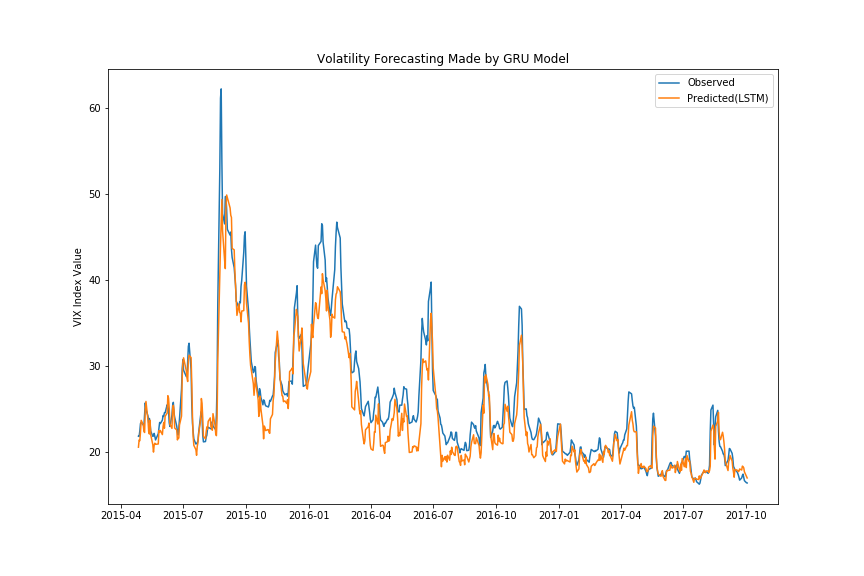
\includegraphics[width=10cm]{GRU.png}
\caption{Observed and Predicted Volatility value without a rolling window}
\end{figure}

\begin{figure}[htbp]
\centering
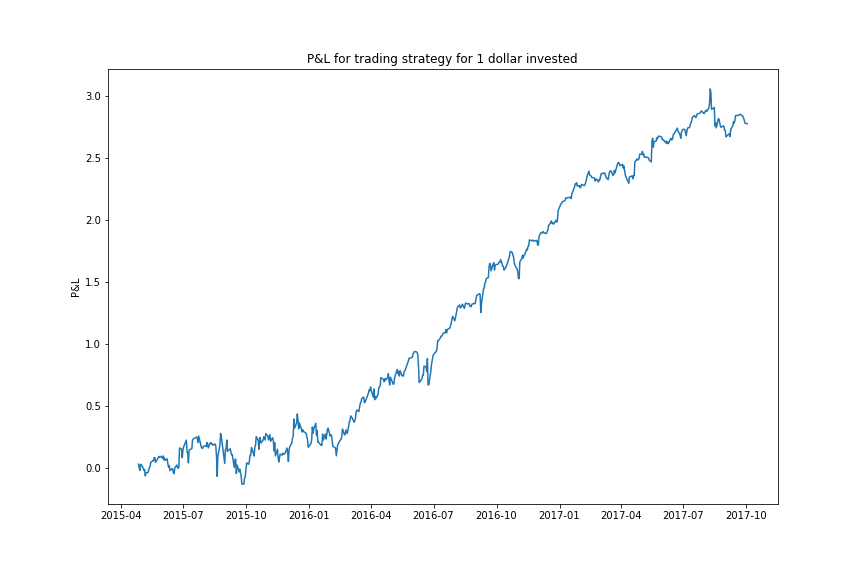
\includegraphics[width=10cm]{Pnl_naive.png}
\caption{Cumulatibe P\&L of naive strategy (without considering transaction cost)}
\end{figure}

\begin{figure}[htbp]
\centering
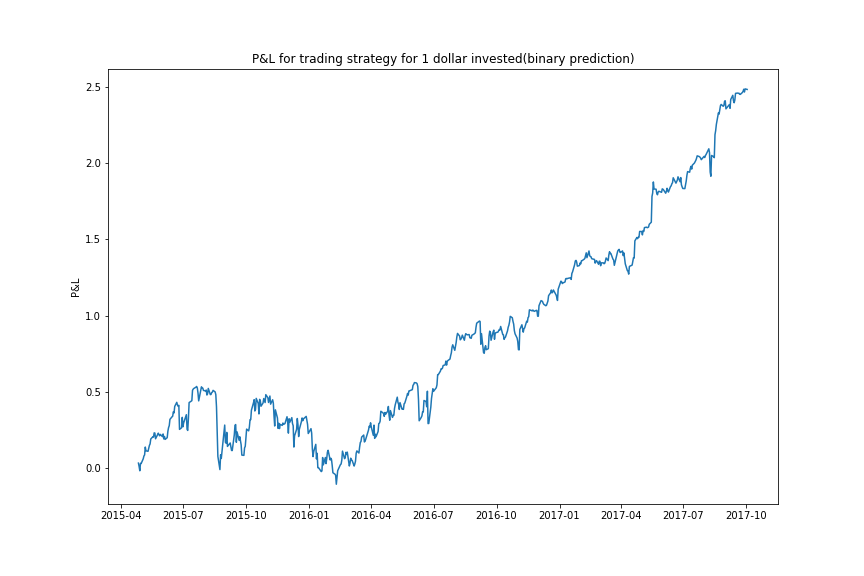
\includegraphics[width=10cm]{Pnl_binary.png}
\caption{Cumulatibe P\&L of the improved strategy (without considering transaction cost)}
\end{figure}

\begin{figure}[htbp]
\centering
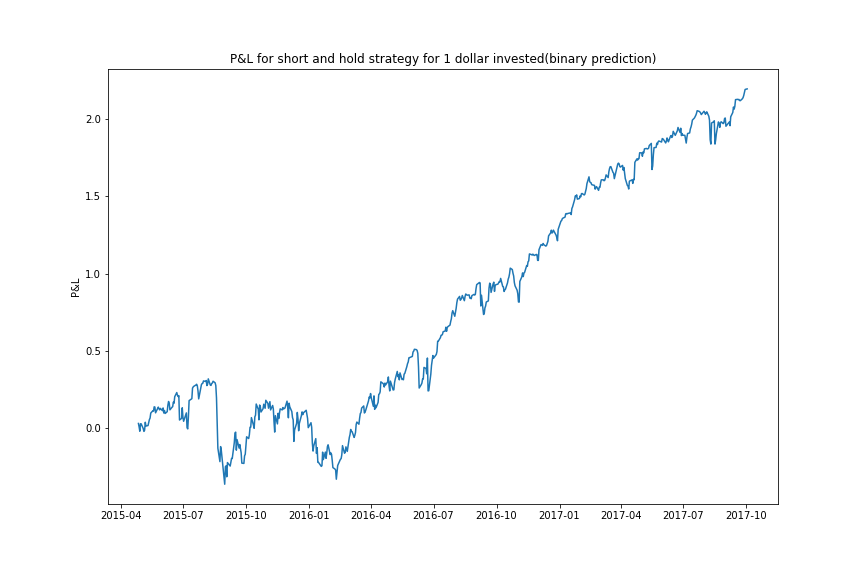
\includegraphics[width=10cm]{Pnl_short.png}
\caption{Cumulatibe P\&L of the short and hold strategy (without considering transaction cost)}
\end{figure}




\end{document}
